%----------------------------------
% PARTIE 2 : Développement du stage
%----------------------------------

\section{Développement du stage}
\label{chp:part2:activities}

\subsection{Prise en main de l’environnement}
\label{sec:taking_environment}

Ma première activité a été la prise en main de l'environnement de travail et
la mise en place d'un setup fonctionnel. Il s'agit ici d'installer les outils
compilant en architecture ARM une première fois le noyau Linux ainsi que le
système opératif sur le support permettant à la STM32MP1 de démarrer, ici en
l'occurence une carte SD.

\subsubsection{Explication de la bootchain}
\label{sec:bootchain_overview}

Avant de booter Linux, un certain nombre d'étapes s'enchevêtre pour passer
d'un état inerte du système à un état où l'utilisateur le prend en main. Cette
séquence transitoire est appelée la bootchain. Lorsque l'utilisateur appuie
sur le bouton de démarrage, un microcode (ou firmware) stocké dans la mémoire
ROM (Read Only Memory), appelé le ROM code, est exécuté par le processeur afin
d'initialiser les horloges primaires. Ce ROM code appele ensuite le premier
étage de boot (FSBL) suivant le mode de démarrage choisi (par carte SD ou lien
en série). Cette étape est primordiale dans la chaîne de boot puisqu'elle doit
être sécurisée dans le but d'empêcher une potentielle vulnérabilité. C'est
pourquoi le ROM code est signé et lui-même authentifie le FSBL. \\

Une fois cet étage de boot chargé en mémoire RAM, celui-ci est exécuté. Lorque
ce dernier prend la main, il termine d'initialiser les horloges et les
premiers composants internes nécessaires au fonctionnement matériel de la
carte. Sur la STM32MP15, le FSBL implémenté est TF-A pour Trusted Firmware -
ARM. TF-A est livré par ARM à destination des processeurs Cortex A7 et A8.
Puis, ce firmware charge et authentifie le second étage de boot SSBL dans la
RAM. \\

Le SSBL instancie les fonctionnalités plus complexes et les périphériques USB,
Ethernet. Il s'occupe également de charger l'image du noyau linux dans la
mémoire vive par l'un des systèmes qu'il instancie (USB, carte SD,
Ethernet...). On pourrait faire une analogie au logiciel GRUB2 qui charge le
noyau Linux sur les architectures x86\_64. \\

Enfin l'image du noyau Linux est exécutée. Les périphériques et mémoires
externes sont reconnues, leurs pilotes instanciés, et les services Unix sont
démarrés. L'utilisateur peut finalement prendre en main la cible. \\

On se rend compte que chaque étape est un processus complexe, sujet à un
développemement ciblé en particulier, TF-A et UBoot étant des projets Open
Source à part entière. Ainsi toutes les versions entre TF-A, UBoot et le noyau
Linux ne sont pas compatibles entre elles. Un problème s'est posé lors du
rajout d'une image du noyau en version de développement 5.4 à un UBoot et un
TF-A à la version délivrée au public antérieure. Il a fallu par conséquent
compiler et écraser manuellement ces deux étages de boot par leurs versions
compatibles. 

\subsubsection{Compilation d'une image du noyau}
\label{sec:kernel_cumpilation}

Le développement du noyau Linux passe obligatoirement par une compilation du
noyau. Celle dernière est faite en plusieurs étapes, épurant le noyau dans un
premier temps, puis configurant l'image et seulement à ce moment, la
compilation et la compression peuvent avoir lieu. La première étape n'est pas
systématiquement nécessaire dans la mesure où les mainteneurs du noyau chez
STmicroelectronics s'assurent constamment d'une rétrocompatibilité.
C'est-à-dire qu'un individu lambda peut compiler un noyau Vanilla (version
sans rajouts ou modifications du noyau) et qui restera fonctionnel sur la
STM32MP15. Cette étape consiste au rajout ou retrait des fragments de
configuration caractéristiques à la carte électronique, qui imposent des
valeurs autres que celles par défaut. En réalité, il s'agit plus d'une étape
de commodité pour les développeurs au sein de l'entreprise pour éviter de
compiler des pilotes des autres architectures et ainsi gagner du temps. \\

\begin{figure}[H]
	\begin{center}
		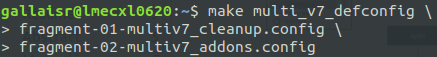
\includegraphics[scale=0.7]{\pathPartTwo/make_multiv7_dark}
		\caption{Commande utilisée pour créer la configuration}
	    \label{fig:make_multiv7}
	\end{center}
\end{figure}

Ensuite, dans le cadre du développement et de tests du noyau, la configuration
avec Kconfig (cf \ref{par:kconfig}) doit s'effectuer afin d'activer les
différents pilotes en cours de développement, comme expliqué ultérieurement.
C'est seulement, après cette étape que la compilation du noyau sera effectuée.
\\

La compilation est effectuée par le Makefile principal, situé dans la racine
du projet. Il fait appel récursivement à tous les Makefiles présents dans
l'arbre du code source. La compilation commence par synthétiser les device
trees, puis une image est formée à partir des pilotes et librairies présentes.
Cet exécutable statique \textbf{vmlinux} n'a pas de format supporté par UBoot
(cf section \ref{sec:bootchain_overview}). Une compression en spécifiant les
adresses des différents secteurs (où l'image doit être copiée dans la RAM,
l'endroit où est situé le binaire dans la partition) est faite comme le montre
l'exemple dans la figure \ref{fig:mkimage} ci-dessous. \\ 

\begin{figure}[H]
	\begin{center}
		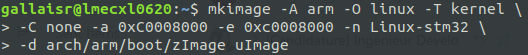
\includegraphics[scale=0.7]{\pathPartTwo/mkimage_dark}
		\caption{Commande utilisée pour créer l'image exploitée par UBoot}
	    \label{fig:mkimage}
	\end{center}
\end{figure}

Cette image finale doit être copiée sur la cible pour que les modifications
faites sur le noyau Linux soient prises en compte. Cela peut être réalisé par
scp si la cible est fonctionnelle et reliée au réseau ou un passage par la
console série UART avec minicom. Cette dernière méthode présente l'avantage
d'évacuer les logs de démarrage et d'exécution sur le terminal de
l'ordinateur. On peut ainsi contrôler les étapes de démarrage et les stopper
au besoin pour prendre la main sur la console des étages de boot. \\

Lorsque toutes ces étapes ont bien été executées, le démarrage de Linux a lieu
et l'utilisateur prend la main sur le système.

\subsection{Intégration de Coresight dans le device tree}
\label{sec:coresight_integration}

Pour instancier les pilotes liés aux composants Coresight pendant le démarrage
du noyau Linux, il faut dans un premier temps les assigner et les implémenter
dans le device tree.  Comme cela est expliqué dans la partie
\ref{sec:coresight_overview}, ces IPs sont internes au SoC, leur
implémentation se fait donc dans un fichier commun qui servira d'inclusion.
La description de ces IPs se fait suivant la \textbf{memory map}. Cela permet
de savoir quels sont les composants accessibles entre eux, où et comment y
accéder. \\

Chaque composant possède ainsi son propre noeud et chaque noeud va ensuite se
décliner en sous-noeuds à la manière du langage de description JSON dont une
analogie pourra être faite. Le noeud spécifie les ports entrées et sorties
présents sur le composant ainsi que des propriétés nécessaires à son
fonctionnement. Elles peuvent faire référence à une horloge, définir une
interruption ou bien être créées sur mesure. Certaines de ces propriétés sont
obligatoires pour permettre au noyau Linux de les reconnaître et de les
inclure. Typiquement, une propriété phare est la propriété \textbf{compatible}
qui associe le noeud dans le device tree à un pilote via une ou plusieurs
chaînes de caractères. Cela se traduit en pratique par une structure de
données dans le pilote appelée par le noyau lors du démarrage. Cette structure
possède un attribut \textbf{name} qui correspond à la chaîne de caractères du
compatible. Par la suite, le pilote appelle une API parser qui décomposera le
noeud en variables et appelera les fonctions en conséquences. \\

Pour prendre l'exemple de l'ETM, illustré en figure \ref{fig:dts_etm}, la
propriété \textbf{compatible} possède deux chaînes de caractères : la première
permet au pilote de reconnaître ce noeud comme étant l'ETMv3 de l'adresse
0x500DC000 ; la deuxième permet d'identifier le composant comme configurable
et non comme un composant passif. \\

Comme la nomenclature a évolué ces trois dernières années, il a fallu corriger
et améliorer le travail effectué en amont. Un avantage de l'Open Source est
que les différentes entreprises upstreament leurs device trees dans le noyau
Linux. On peut implémenter par conséquent le système présent en faisant des
analogies aux autres device trees par méthodologie comparative. \\

Implémenter le sous-système Coresight dans le device tree ne règle pas le
problème de son activation. Comme cela est expliqué dans la section
\ref{par:dt}, les noeuds Coresight du device tree ne sont appelés que par les
pilotes Coresight.  S'ils ne sont pas eux-mêmes compilés et intégrés dans
l'image du noyau Linux, leur appel n'aura pas lieu lors du boot, et les IPs
Coresight resteront dormants. Dans la configuration du noyau, les développeurs
ont créé le système de configuration Kconfig (cf section \ref{par:kconfig}).
Dans les options de configuration apparaît la macro CORESIGHT qui active
l'utilisation du système.  Des sous-options sont alors déclinées, permettant
affinant la configuration.  On peut par la suite choisir d'activer les pilotes
pour chaque composant. \\

\subsection{Décodage des premières trames Coresight}
\label{sec:coresight_traces}

\subsubsection{Choix du décodeur}
\label{sec:decoder_choice}

Pour comprendre la suite de cette section, une parenthèse est nécessaire pour
expliquer le fonctionnement des traces Coresight véhiculées au niveau
matériel. Ce flux de données, nommé \textbf{Program Flow Trace}, est généré
par les composants sources, et arrive dans un buffer ou bien est évacué par un
port JTAG. Le Program Flow Trace construit des trames à partir de différentes
instructions que le processeur effectue. En connaissance de ces étapes, en
plus de l'image du noyau Linux, on reproduit ce que le processeur a accompli,
et ainsi retrace le code exécuté à posteriori.  Seulement comme lors d'un
enregistrement, il peut se passer une infinité d'évènements (en admettant que
l'on fasse appel à un programme contenant une boucle infinie), une compression
est donc nécessaire afin de ne pas saturer le buffer de sortie. Il faudra
envisager de décoder ces traces binaires. \\

Une alternative fut prise concernant le décodage de ces traces. En effet, il
existe de nombreuses solutions, différentes les unes par rapport aux autres,
et chacune apportant ses avantages. On recense ainsi les solutions suivantes : 

\begin{itemize}[label=\textbullet]
    \item Trace32/Lauterbach
    \item DS-5
    \item ptm2human
    \item OpenCSD
\end{itemize}

L'utilisation d'un \textbf{Lauterbach}, sonde de débogage, se révèle très
pratique pour l'observation invasive du système. Cet instrument s'accompagne
d'un logiciel, \textbf{Trace32}, qui évacue des traces et les analyse
directement par le port JTAG. Cependant, c'est une technologie très coûteuse et
non accessible aux personnes de la communauté Linux. C'est pour cela qu'il n'y
a que 2 Lauterbachs sur le site de ST Le Mans et de surcroît, cette solution
n'est pas adaptée pour ce projet. De même, \textbf{DS-5} est un logiciel
propriétaire ARM de développement supportant de décodage de trace Coresight.
Une édition communautaire existe, mais elle n'implémente pas nativement ce
décodage. Il y reste donc comparativement deux dernières solutions. Ce
sont des libraires Open Source que l'on peut retrouver sur GitHub. Lorsque
l'on s'attarde sur leur code source, on se rend compte qu'\textbf{OpenCSD} est
toujours active tandis que \textbf{ptm2human} n'est plus maintenue en
apparence. Cette dernière librairie a ainsi potentiellement une obsolescence
que l'on ne retrouve pas chez OpenCSD.  Par ailleurs, OpenCSD s'intègre à
perf et permet une compilation sur cible.  C'est naturellement vers cette
solution que le projet s'est orienté pour décoder les traces Coresight.

\subsubsection{Mise en place du décodage}
\label{sec:proper_decoding}

La librairie choisie est compilée au format ARM 32 bits et x86\_64 pour
décoder des traces sur cible et sur ordinateur hôte. Une fois la librairie
enregistrée dans la toolchain aux formats ELF 32 et 64 bits, l'intégration à
l'outil perf pour chaque architecture est effectuée. Cela se fait par le
passage d'une option dans les arguments du Makefile comme le montre la figure
\ref{cmd:perf_compilation}. Cela retourne un exécutable ELF dynamiquement lié
au format 32 bits. Il ne reste plus qu'à copier les librairies et l'exécutable
sur la cible, si la commande ci-dessous a été exécutée dans l'environnement de
développement ARM. 


\begin{figure}[H]
	\begin{center}
		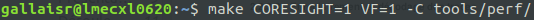
\includegraphics[scale=0.7]{\pathPartTwo/make_perf_dark}
		\caption{Commande utilisée pour compiler perf}
            \label{cmd:perf_compilation}
	\end{center}
\end{figure}

\subsubsection{Enregistrement et décodage des traces}

L'enregistrement et le décodage de traces se font par deux commandes :

\begin{itemize}[label=\textbullet]
	\item \textbf{perf record}
	\item \textbf{perf report}
\end{itemize}

La première commande génère un binaire \textbf{perf.data} contenant toutes les
traces et les évènements reçus par le framework durant la commande exécutée.
Elle stocke également les librairies et modules utilisés par le noyau lors de
son exécution dans un dossier, généralement \textbf{\$HOME/.debug/}. La
seconde interprète le fichier et le dossier qu'elle affiche dans une interface
utilisateur. \\

L'intérêt de \textbf{perf record} réside dans l'enregistrement des traces
suivants plusieurs critères bien définis qui modifient l'origine de la trace,
les secteurs à enregistrer ou encore le format de la trace. 

\begin{figure}[H]
	\begin{center}
		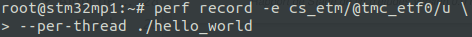
\includegraphics[scale=0.7]{\pathPartTwo/perf_record_dark}
		\caption{Commande utilisée pour enregistrer des traces}
            \label{cmd:perf_record_cs_etm}
	\end{center}
\end{figure}

Dans l'exemple ci-dessus, on cherche à mettre en évidence les différents
appels fait par la fonction \textbf{printf} aux librairies C au sein du
programme \textbf{hello\_world}. L'option \textbf{-e} désigne l'évènement qui
doit être surveillé et enregistré. Néanmoins, cette option est requise pour
utiliser le framework Coresight. Elle sélectionne en réalité l'évènement que
la PMU doit gérer.  Intrinsèquement, cela appelle l'abstraction de la PMU
faite par le framework Coresight (cf \ref{sec:perf_coresight_framework}).
\textbf{cs\_etm} identifie le composant générateur de trames Coresight et
\textbf{@tmc\_etf0} spécifie le point d'arrivée des trames. L'utilisateur peut
préférer de limiter l'enregistrement des évènements dans l'espace utilisateur
ou l'espace noyau grâce aux options \textbf{u} ou \textbf{k}. Par défaut,
lorsque cette option n'est pas spécifiée, les évènements survenant dans les
deux domaines sont capturés.  Enfin, il y a la possibilité d'effectuer des
traces suivants les threads du programme surveillé avec \textbf{--per-thread}
ou contrôler l'ensemble des CPUs avec \textbf{--all-cpus}. \\

Pour reprendre l'exemple, on enregistre ainsi les appels de fonctions de
l'espace utilisateur du programme \textbf{hello\_world} en triant ces appels
en fonction des différents threads. \\

Une fois les traces enregistrées dans le fichier \textbf{perf.data},
\textbf{perf report} affiche le profil de performance. Encore une fois,
différentes options s'offrent à l'uilisateur pour le choix de l'interface. Une
présentation des données brutes peut être faite avec :

\begin{figure}[H]
	\begin{center}
		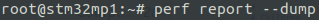
\includegraphics[scale=0.7]{\pathPartTwo/perf_report_dump_dark}
		\caption{Commande utilisée pour observer des traces brutes}
            \label{cmd:perf_report_dump}
	\end{center}
\end{figure}

Malgré des informations peu lisibles, cette fonction a l'avantage de présenter
directement les trames Coresight mémorisées. \\

\begin{figure}[H]
	\begin{center}
		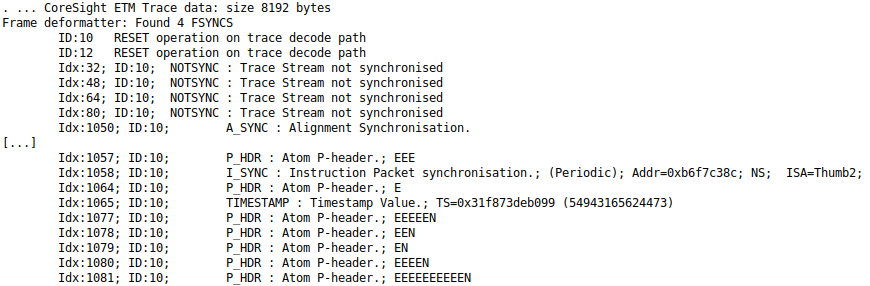
\includegraphics[width=\textwidth]{\pathPartTwo/perf_data_dump}
		\caption{Extrait du fichier perf.data à la section perf}
	    \label{fig:perf_data_dump}
	\end{center}
\end{figure}

Parmi les 8 kilooctets de données collectées, plusieurs trames sont
remarquables :

\begin{itemize}[label=\textbullet]
    \item A\_SYNC : Ce packet permet au décodeur d'aligner les trames avec leur
        adresse. Il permet au décodeur d'identifier les différents packets.
    \item Atomes P\_HDR : Ces paquets composés d'atomes, indiquent l'exécution
        des instructions. Un atome peut prendre la valeur :
        \begin{itemize}
            \item \textbf{E} indiquant que l'instruction est passée.
            \item \textbf{N} indiquant que l'instruction n'est pas passée.
            \item \textbf{W} est une valeur particulière, qui n'est pas
                applicable ici.
        \end{itemize}
    \item BRANCH\_ADDRESS (non visible sur la figure \ref{fig:perf_data_dump})
        : Les branchements sont des instructions venant interrompre
        l'exécution séquentielle d'un processeur. Ce paquet spécifie
        lorsqu'une opération de branchement survient ainsi que l'adresse de la
        prochaine instruction à exécuter.
    \item I\_SYNC : Ce packet synchronise les instructions, il renvoie
        l'adresse de l'instruction courante.
    \item TIMESTAMP (non visible sur la figure \ref{fig:perf_data_dump}) : Le
        Timestamp est une valeur arbitraire envoyée à intervalles réguliers.
        Il sert à identifier lorsque plusieurs flux de données sont présents,
        par exemple lors d'une trace sur plusieurs processeurs.
    \item CtxtID (non visible sur la figure \ref{fig:perf_data_dump}) : Ces
        paquets sont envoyés pour avertir du changement de contexte au sein du
        processeur. Ce paquet comporte l'identifiant du nouveau contexte.
\end{itemize}

Par ailleurs, chaque packet présente l'identifiant du processeur sur lequel il
est récupéré. \textbf{ID:10} désigne le premier processeur A7, et
\textbf{ID:12} désigne le second processeur. Sur la figure
\ref{fig:perf_data_dump}, on a donc une exécution du programme qui ne s'est
réalisée que sur un coeur du SoC. \\

De même, il existe une présentation plus orientée utilisateur avec :

\begin{figure}[H]
	\begin{center}
		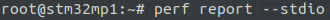
\includegraphics[scale=0.7]{\pathPartTwo/perf_report_stdio_dark}
		\caption{Commande utilisée pour observer des traces formatées}
            \label{cmd:perf_report_stdio}
	\end{center}
\end{figure}

L'option \textbf{--stdio} affiche le résultat comme un texte. Par défaut,
l'application utilise la librairie graphique NCurses. Dans une mesure de
simplification de la présentation, on utilise le format texte. \\

\begin{figure}[H]
	\begin{center}
		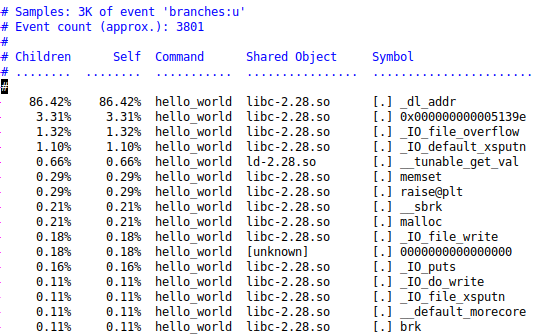
\includegraphics[width=\textwidth]{\pathPartTwo/perf_data_stdio}
		\caption{Extrait du fichier perf.data à la section perf}
	    \label{fig:perf_data_sdtio}
	\end{center}
\end{figure}

Sur l'image \ref{fig:perf_data_sdtio} ci-contre on observe donc les
différentes fonctions appelées par la commande supervisée. \\

L'aperçu du résultat montre d'abord une approximation du nombre d'évènements
reçus. Puis, sont affichées 5 colonnes chacune ayant une signification bien
précise.  Les deux premières colonnes \textbf{Children} et \textbf{Self}
désignent le pourcentage de temps passé dans la fonction appelée par rapport
au temps total d'exécution. La somme de ces pourcentages est normalement égale
à 100\% pour la colonne "Self", tandis que ce n'est pas un cas systèmatique
pour "Children". Cela est dû au calcul du temps. Children représente la somme
du temps passé dans les processus fils. La troisième colonne, explicite,
précise qu'elle était la commande supervisée lors de l'appel. Dans le cas
présent, c'est le programme \textbf{hello\_world}. La quatrième et la dernière
colonne font respectivement référence à la librairie utilisée et la fonction
appelée, appelée aussi symbole, dans cette librairie. Dans le cas où le
symbole n'est pas reconnu, perf pointe vers son adresse. Lorsque l'échantillon
mesuré provient du noyau, la référence à la librairie est remplacée par
\textbf{[kernel.kallsyms]} et le \textbf{[.]} signifiant l'espace utilisateur
du symbole est remplacé par \textbf{[k]}.

\subsection{État de l'art du débogage interprocesseurs}
\label{sec:faisabilite_m4}

Une étude annexe a consisté à faire un état de l'art concernant le débogage
interprocesseurs. \\

L'Evalboard possède 3 coeurs : 2 processeurs ARM Cortex-A7 et un coprocesseur
ARM Cortex-M4. Généralement, les coeurs des deux processeurs délèguent les
tâches de calculs au coprocesseur. Cela explique l'idée de vouloir déboguer le
troisème coeur par l'intermédiaire des coeurs A7. Cette mission a ainsi pour
objet de vérifier si l'utilisation des IPs Coresight pour récupérer les traces
du Cortex-M4 est possible. \\

Pour comprendre la stratégie de développement, une discussion avec Mathieu
Poirier, expert Linaro a été entamée. Ce dernier a expliqué que, dans le cas
où l'ETM appartenant au domaine du coprocesseur était accessible depuis l'un
des deux processeurs Cortex-A7, il suffisait seulement à le configurer pour
l'activer.  Cela serait possible puisque les traces qu'il produit atterrissent
directement dans le ETF, buffer de sortie commun avec les traces des deux
coeurs A7. \\

Aussi dans un premier temps, il a fallu comprendre si les différents registres
de l'ETMv3 du coprocesseur étaient accessibles depuis les deux coeurs ARM
Cortex-A7.
 
\subsubsection{Analyse préliminaire}
\label{sec:initial_analysis}

Les processeurs et le coprocesseurs n'appartiennent pas au même domaine dans
la mémoire. Leurs registres et périphériques associés sont séparés, et les
accès mémoires passent par l'intermédiaires de bus de données ne communiquant
pas directement. Dans le domaine des processeurs, les composants Coresight
utilisent le bus \textbf{APB-D} tandis que ceux du coprocesseur utilisent le
bus \textbf{AHB}. Des ports permettant des échanges sont accessibles à
différents bus et permettraient d'accéder aux registres des composants
Coresight du coprocesseur. Ces deux ports \textbf{AHB-AP} pour le bus AHB et
le port \textbf{APB-AP} pour le bus APB-D communiquent par un troisième, le
\textbf{DAPBUS} que la figure \ref{fig:bus_ports} met en valeur.  Dans une
mesure de sécurité, la communication entre ces différents bus n'est possible à
condition qu'un espace mémoire pour les IPs soit implémenté dans chaque bus,
et que des signaux d'authentification soient activés par le \textbf{BSEC}.  \\

\begin{figure}[H]
	\begin{center}
		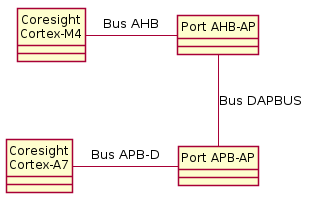
\includegraphics[scale=0.7]{\pathPartTwo/bus_ports}
		\caption{Diagramme d'accès aux bus}
	    \label{fig:bus_ports}
	\end{center}
\end{figure}

Ce périphérique interne est destiné à configurer le SoC et ses paramètres de
sécurité via le contrôle d'une puce. En particulier, il possède un registre
\textbf{BSEC\_DENABLE} définissant les signaux d'authentification nécessaires
au déboguage du SoC qui seront utilisés. Parmi les signaux utiles, on retrouve
:

\begin{itemize}[label=\textbullet]
    \item DBGEN (bit 1) qui active le débogage.
    \item NIDEN (bit 2) qui active le débogage non-invasif.
    \item DEVICEEN (bit 3) qui autorise l'accès aux composants Coresight par
        un port extérieur.
    \item DBGSWENABLE (bit 10) qui active l'accès logiciel aux composants
        Coresight.
\end{itemize}

Ce registre est accessible à l'adresse 0x5C005014 grâce à un utilitaire
similaire à busybox, \textbf{devregs} qui lit et écrit à l'adresse donnée si
le registre le permet. La lecture du registre renvoie 0x0000047F. Les signaux
listés sont donc activés et la valeur renvoyée laisse penser par conséquent
que l'implémentation d'une solution pour un dégogage interprocesseurs est
possible.

\subsubsection{Ajout de l'ETM du coprocesseur au device tree}
\label{sec:add_etm_m4_dt}

Intuitivement et aux vues de la description qu'il a fallu ajouter et modifier
dans le device tree, une première étape fut d'instancier l'ETM dans le device
tree, à l'instar des deux ETM dédiés aux processeurs Cortex-A7. L'ETM du
coprocesseur se situe à l'adresse 0xE0041000 dans la memory map. \\

L'instanciation de l'ETM est faite dans le device tree à l'adresse indiquée
ainsi que les branchements au funnel pour pousser les traces en sortie (cf
\ref{fig:debug_support_structure_diagram}). Une fois le noyau Linux démarré,
on vérifie l'état de l'ETM ; ce qui est fait par la lecture avec devregs du
premier registre des ETMs du coprocesseur, de valeur initiale 0x00000411 et
d'un processeur en tant que témoin, l'\textbf{ETMCR} qui possède un offset en
mémoire de 0x000 et une valeur par défaut de 0x00000461. Celui-ci montre la
valeur 0xbff5f77b, différente de celle par défaut (0x00000411) tandis que
l'ETM du processeur vaut bien la valeur par défaut (0x00000461). \\

Le coprocesseur étant dormant à ce niveau de l'étude, cela expliquerait le
comportement de l'ETM. Un firmware est téléversé sur le microcontrôleur afin
de le démarrer avant le noyau Linux. Cependant, malgré l'activation du
microcontrôleur, le démarrage du noyau est impossible en raison d'une erreur
persistante. Cette erreur engendre un blocage lors de l'initialisation d'un
périphérique du STM32MP15 qui ne peut alors plus démarrer.

\subsubsection{Vérification dans la memory map}
\label{sec:mmap}

En regardant sur la memory map de la puce électronique, on se rend compte que
l'adresse normalement occupée par l'ETM du coprocesseur est réservée à la
mémoire DDR, et que seul le débogueur peut accéder à cette adresse. Une
explication possible de la valeur en apparence arbitraire du registre
s'expliquerait par une lecture dans une zone réservée de la mémoire. La memory
map montre également qu'il n'y a pas d'emplacement dédié à l'ETM du
coprocesseur parmi les bus de communication des processeurs. \\

L'étude menée se révèle ainsi non concluante car les IPs Coresight du
coprocesseur ne sont pas accessibles depuis les processeurs. Un phénomène
intéressant en revanche est notable : les accès mémoires autorisent une
lecture/écriture des registres des IPs Coresight dédiés aux Cortex-A7 depuis
le coprocesseur.  \\

Dans un second temps, on souhaiterait partir de la communication existante
entre le A7 et le coprocesseur pour lancer une trace sur le M4 et recevoir les
infos de débogage par les processeurs. Le coprocesseur, non autonome pour
cette partie-là, serait alors un "esclave" des processeurs. \\

Au sein du noyau Linux, il existe un système de boîte aux lettres, appelé
remoteproc, par lequel les processeurs et le coprocesseur communiquent.  Comme
le montre la figure \ref{fig:coprocessor_management} suivante, cette
communication se base sur une mémoire partagée entre les trois coeurs du
système. Il faudrait ainsi créer un protocole de communication spécifique pour
du débogage avec Coresight et implémenter dans la HAL (Hardware Abstraction
Layer) des pilotes configurant les registres des IPs Coresight. Le
coprocesseur activerait par la suite son système selon la demande faite par
remoteproc et enverrait les évènements et les traces à l'ETF pour qu'il les
intégre. \\

\begin{figure}[H]
	\begin{center}
		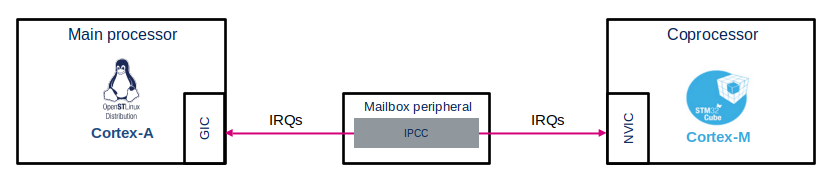
\includegraphics[width=\textwidth]{\pathPartTwo/coprocessor_management}
		\caption{Diagramme fonctionnel de l'infrastructure Remoteproc}
	    \label{fig:coprocessor_management}
	\end{center}
\end{figure}

Une solution pourrait être ainsi implémentable sur une vision au long terme.
Un tel développement, en prenant en compte la conception du protocole de
communication, l'implémentation des pilotes Coresight du coprocesseur dans le
cas où ils n'existent pas, prendrait entre deux à trois ans à temps plein pour
deux ingénieurs (un ingénieur par tache). En considérant l'intégration de ce
système avec perf, il faudrait au moins deux ans supplémentaires pour arriver
à un système fonctionnel. L'idée de déboguer le coprocesseur est donc
abandonnée pour ce projet.

\subsection{Ajout de fonctionnalité à perf}
\label{sec:add_perf_feature}

En étudiant le code source des pilotes Coresight, le TPIU apparaît comme
incomplet. Celui-ci étant un \textbf{pilote bouchonné}, par conséquent qui ne
fait rien d'autre que de renvoyer un résultat prédéfini ou une erreur, il
aurait été judicieux de l'implémenter. En effet, cette IP débouche sur le port
JTAG. À moyen terme pour valider le travail effectué, il aurait fallu passer
par un décodage des traces avec \textbf{Lauterbach}. Comme cela a été évoqué
en section \ref{sec:decoder_choice}, peu de clients risquent de l'utiliser en
raison de son coût. Aussi, l'implémentation de ce pilote a été abandonnée.
Néanmoins, au cours de l'étude de faisabilité, une erreur a été detectée lors
de la collecte d'une trace. Effectivement, lors d'une trace au niveau du noyau
avec un échantillonage de tous les CPUs (directive \textbf{--all-cpus}), un
crash de perf est observé.  En regardant les appels systèmes de perf avec
l'utilitaire \textbf{strace}, on observe la lecture d'un registre d'un ETMv4
avant le crash de l'application.

\subsubsection{Problématique d'implémentation}
\label{sec:problem_implementation}

Cette référence aux registres de l'ETMv4 est due en partie au travail effectué
autour du framework Coresight et de son intégration dans perf. En effet,
l'ETMv4 n'est pas une version supportée par un processeur Cortex-A7, mais par
un Cortex-A8, plus puissant que le Cortex-A7. La demande client auprès de ce
processeur étant plus grande, les développeurs s'attardent plus sur ce
processeur et ses périphériques. De plus le Cortex ARM V8 n'est compatible
qu'avec l'ETM en version 4. \\

L'utilisation intensive du débogueur GDB sur les cas générants un crash de
perf a permit l'identification d'un problème : le traitement de l'ETMv3 est
écarté. Le code source de perf se voulant générique, la création d'un objet
\textbf{cs\_etm} autorise une interface standard entre perf et les différentes
versions des ETM dans l'espace utilisateur. C'est donc cet objet que perf
appelle lors de l'échantillonage des traces et qui effectue les appels
systèmes au noyau en conséquences. L'objet configure par la suite une
structure de données selon la version de l'ETM et retourne un pointeur vers
cette structure. \\

Au sein de cet objet, un test est passé pour connaître l'origine de l'ETM en
fonction de l'identifiant du CPU qui lui est donné en argument. Puis, la
configuration diffère suivant le booléen retourné. Ce test est effectué dans
la fonction \textbf{cs\_etm\_is\_etmv4}, dont on peut voir le prototype
ci-dessous.

\begin{lstlisting}[language=C]
static bool cs_etm_is_etmv4(struct auxtrace_record *itr, int cpu)
\end{lstlisting}

Dans cette fonction, l'interface sysfs est utilisée pour scanner les fichiers
des registres en lecture seule. Suivant la présence ou non d'un fichier
correspondant à un registre spécifique de l'ETMv4, une valeur est renvoyée.
C'est ensuite en fonction de ce booléen qu'une erreur est renvoyée par le
programme. Considéré comme étant critique dans la configuration de perf, rien
n'est enregistré et la commande s'arrête. Cette fonction est notamment appelée
dans les fonctions responsables de la configuration du \textbf{ContextID} et
du \textbf{Timestamp}. \\

Cette gestion de l'ETMv3 non implémentée explique ainsi le comportement de
perf lors de l'échantillonage de tous les CPUs. 

\subsubsection{Comparaison entre les registres de l'ETMv3 et l'ETMv4}
\label{sec:etmv3_etmv4_comparison}

Pour comprendre la logique d'implémentation, et notamment quelles sont les
fonctions des registres de l'ETMv4 qui ont été gérées, une étude comparative
entre les registres de l'ETMv4 et l'ETMv3 utilisés a été menée. Ces registres
apparaissent dans le sysfs en lecture seule à titre informatif de l'état et
des capacités de l'ETM. La lecture dans l'interface sysfs est obligatoire
puisque la partie espace utilisateur du code de perf ne peut pas accéder
directement aux registres.

\paragraph{Timestamp}\mbox{}\\
\label{par:timestamp}

\begin{lstlisting}[language=C]
static int cs_etm_set_timestamp(struct auxtrace_record *itr,
				struct evsel *evsel, int cpu)
\end{lstlisting}

Dans la fonction de gestion du timestamp ci-dessus, le registre
\textbf{TRCIDR0} de l'ETMv4 est lu par l'interface sysfs, puis stocké dans une
variable. Ce registre de 32 bits en lecture seule indique les capacités de
traçage de l'ETMv4. Il possède notamment un mot \textbf{TSSIZE} de 5 bits
consacré à la taille du timestamp. Ce mot peut prendre 3 valeurs :

\begin{itemize}[label=\textbullet]
    \item 0 (0b00000 en binaire) dans le cas où le timestamp n'est pas
        supporté
    \item 6 (0b00110) pour signifier que le timestamp sera encodé sur 48 bits.
    \item 8 (0b01000) pour signifier que le timestamp sera encodé sur 64 bits. 
\end{itemize}

\begin{figure}[H]
	\begin{center}
		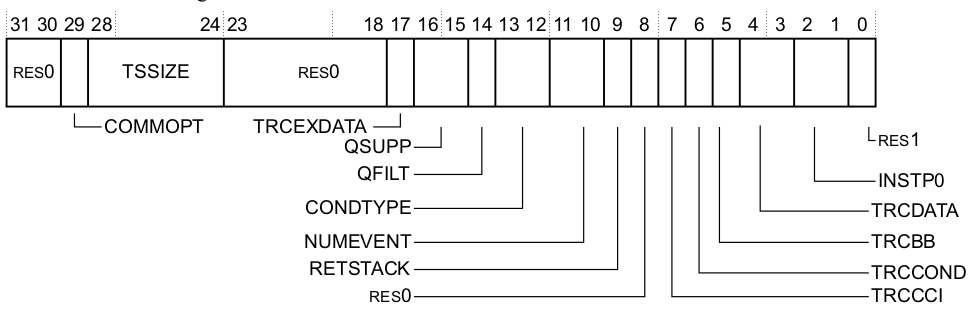
\includegraphics[width=\textwidth]{\pathPartTwo/etmv4_trcidr0_register}
		\caption{Aperçu du registre TRCIDR0 de l'ETMv4}
	    \label{fig:etmv4_trcidr0_register}
	\end{center}
\end{figure}

Par la suite dans la fonction de configuration du timestamp, un
\textbf{masque} de la taille du mot \textbf{TSSIZE} est appliqué sur la
variable contenant la valeur du registre afin de l'isoler. Elle est testée
dans une condition pour connaître si l'ETM supporte le traçage du timestamp.
Enfin elle avertie le noyau Linux de la configuration. Dans le cas contraire
la fonction renvoie une erreur. \\

Dans la documentation du SoC, un registre de l'ETMv3 est en rapport avec le
Timestamp : \textbf{ETMCCER} (ETM Configuration Code Extension Register).  Il
possède le même champ \textbf{TSSIZE} que le registre de l'ETMv4 et le champ
\textbf{TIMSTMP}. À la différence de l'ETMv4, ces mots sont encodés sur 1 bit.
De plus, c'est TIMSTMP qui définit si le timestamp est supporté, TSSIZE ne
fait qu'indiquer la taille du tmestamp. Ainsi si TIMSTMP vaut 0, la
fonctionnalité de timestamp n'est pas implémentée.

\begin{figure}[H]
	\begin{center}
		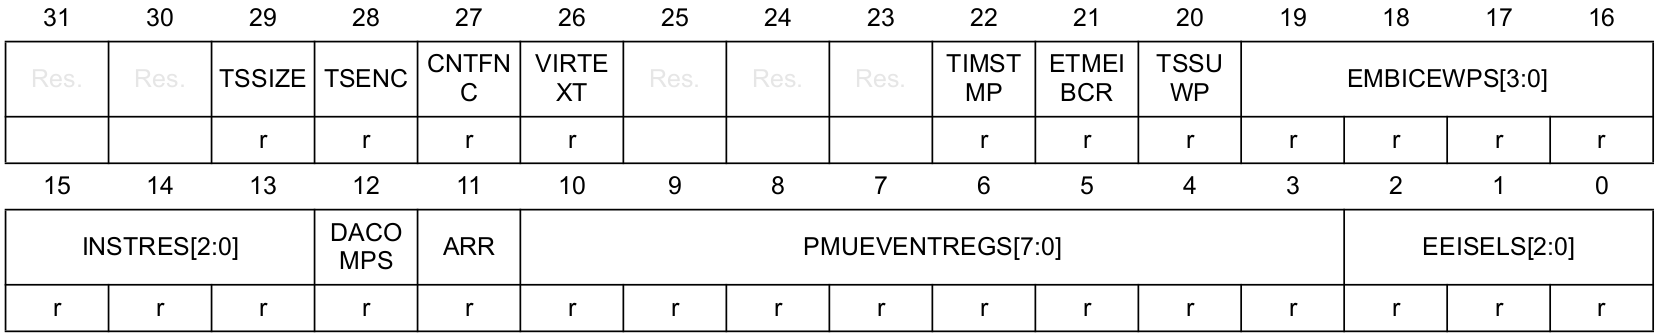
\includegraphics[width=\textwidth]{\pathPartTwo/etmv3_etmccer_register_2}
		\caption{Aperçu du registre ETMCCER de l'ETMv3}
	    \label{fig:etmv3_etmccer_register}
	\end{center}
\end{figure}

Comme ce registre apparaît en lecture seule, il est immuable. Une vérification
de sa valeur en passant par sysfs montre que le bit 22 correspondant à
\textbf{TIMSTMP} est à 1. L'ajout du registre est donc possible. Pour ce
faire, le retour d'erreur précédemment cité en section
\ref{sec:problem_implementation} est remplacé par la lecture de ce registre,
puis une condition est ajoutée pour effectuer le traitement de la valeur du
registre et l'avertissement de la configuration au noyau Linux. Ce
séquencement est illustré par la figure \ref{fig:cs_etm_set_context_id},
commun avec la section suivante.

\paragraph{Context ID}\mbox{}\\
\label{par:contextid}

\begin{lstlisting}[language=C]
static int cs_etm_set_context_id(struct auxtrace_record *itr,
				 struct evsel *evsel, int cpu)
\end{lstlisting}

La fonction de la configuration du Context ID se comporte d'une manière
similaire à la fonction liée au timestamp. Le registre utilisé a plusieurs
taches, dont celle d'indiquer la taille de l'adresse de l'instruction exécutée
et celle d'indiquer la taille du Context ID. Cette dernière tache est
appréhendée par un mot \textbf{CIDSIZE} de 5 bits sur le deuxième octet du
registre (figure \ref{fig:etmv4_trcidr2_register}). Lorsque la valeur de ce
mot vaut 0 (0b00000 en binaire), le ContextID n'est pas supporté par l'ETMv4 ;
donc il ne créera pas ce paquet dans le flux de traces. Dans le cas où il vaut
4 (0b00100 en binaire), cela signifie que le Context ID est supporté et que sa
taille peut atteindre 32 bits au maximum. Les autres valeurs de cet octet sont
ignorées. L'information utile de ce registre est de montrer que le Context ID
est supporté sur l'ETM. 

\begin{figure}[H]
	\begin{center}
		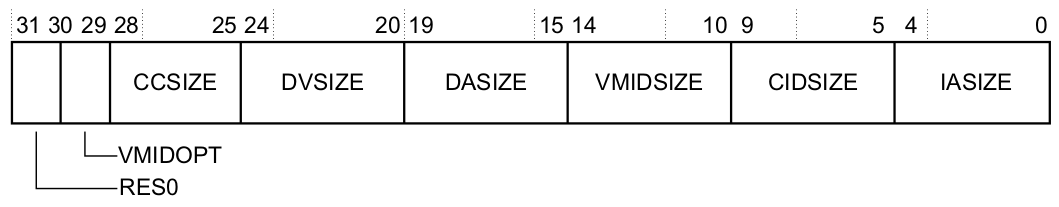
\includegraphics[width=\textwidth]{\pathPartTwo/etmv4_trcidr2_register}
		\caption{Aperçu du registre TRCIDR2 de l'ETMv4}
	    \label{fig:etmv4_trcidr2_register}
	\end{center}
\end{figure}

Deux registres dans l'ETMv3 y réfèrent et potentiellement pourraient être
l'analogue du registre TRCIDR2 dans l'ETMv4. \\

Le premier, dont on reviendra en section \ref{sec:clocks_and_tsgen}, est le
registre de contrôle général de l'ETM : \textbf{ETMCR} (ETM Control Register).
Ce registre en lecture/écriture possède un champ de 2 bits dédié à la taille
du Context ID. Il peut prendre les valeurs suivantes :

\begin{itemize}[label=\textbullet]
	\item 0 ou 0b00
	\item 1 ou 0b01 
	\item 2 ou 0b10 
	\item 3 ou 0b11 
\end{itemize}

Dans le cas où ce champ vaut 0, le Context ID n'est pas supporté. Dans les
autres cas, cela indique quelles sont les tailles du Context ID. \\

Le second registre est un registre de configuration en lecture seule :
\textbf{ETMCCR} (ETM Configuration Code Register). La documentation précise
qu'il "permet au logiciel de lire la configuration [...] de l'ETM, donnant le
nombre de chaque type de ressource". À l'instar de l'ETMCR, il possède un mot
\textbf{CONTXTIDCMP} de 2 bits, et indique le nombre de comparateurs utilisés
(pouvant aller jusqu'à 3) pour créer le Context ID. Si sa valeur est à 0, il
n'y a pas de comparateurs et le Context ID n'est pas supporté. Dans le
STM32MP15, il n'y a qu'un comparateur, la valeur du CONTXTCMP affichée par
défaut dans sysfs est 1 (0b01).

\begin{figure}[H]
	\begin{center}
		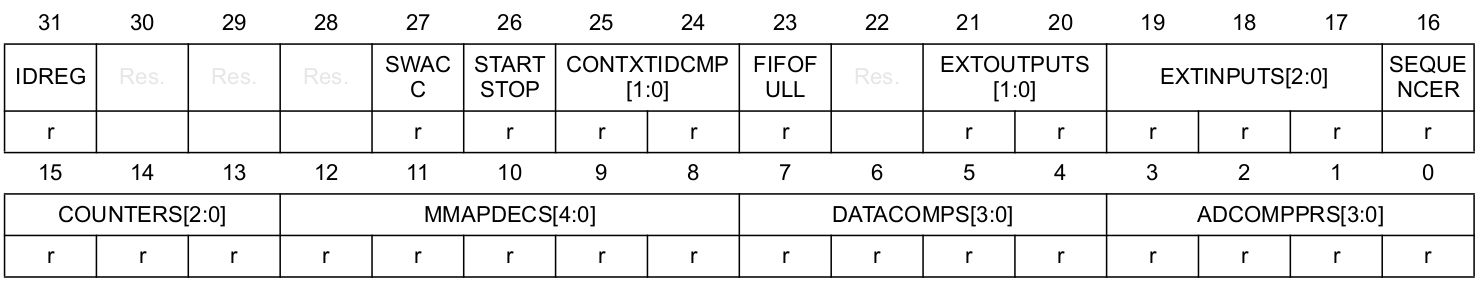
\includegraphics[width=\textwidth]{\pathPartTwo/etmv3_etmccr_register_2}
		\caption{Aperçu du registre ETMCCR de l'ETMv3}
	    \label{fig:etmv3_etmccr_register}
	\end{center}
\end{figure}

L'\textbf{ETMCR} est d'abord implémenté de la même manière que le registre de
l'ETMv4 \textbf{TRCIDR2} en prenant compte de la gestion d'erreur. Un échange
avec Mathieu Poirier pour discuter de l'implémentation révèle que le mot
CONTXTIDSIZE de l'ETMCR est un masque de bit à tracer et non à lire.
C'est-à-dire que l'écriture dans ce registre affecte la configuration
générale de l'ETM, comme son nom l'indique. L'implémentation avec ce registre
ainsi abandonnée, puis remplacée avec l'\textbf{ETMCCR}. Au final, les deux
fonctions modifiées ressemblent à la figure \ref{fig:cs_etm_set_context_id}
ci-dessous. \\

Une campagne de tests montre que les traces enregistrées proviennent bien des
deux processeurs Cortex-A7. Cela est fait par l'exécution d'un programme en
espace utilisateur contenant deux threads. Pour s'assurer que ces deux threads
s'exécutent bien sur les deux coeurs et non en alternance sur un seul coeur,
leur affinité est associée pour chaque coeur, dans un premier temps. Ensuite,
après avoir vérifié que l'affinité de Linux exploite bien tous les coeurs
présents par défaut, un simple programme exécutant deux threads est utilisé
dont le code source se trouve en annexe. \\

\underline{\textbf{Note : }} Sur le diagramme ci-dessous est représenté en
bleu les étapes déjà implémentées et en beige les étapes qui ont été ajoutées. 

% trace.affinity.all-cpus.2020_06_05_150756.tgz

\begin{figure}[H]
	\begin{center}
		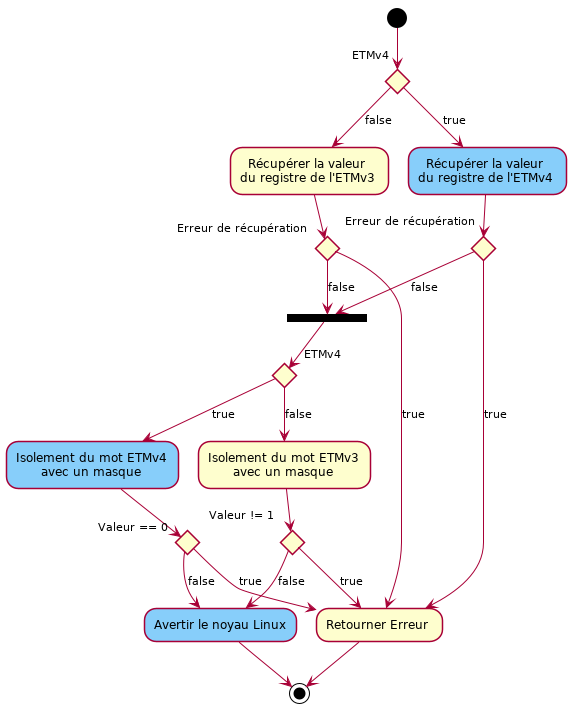
\includegraphics[scale=2.5]{\pathPartTwo/cs_etm_set_context_id}
		\caption{Algorithme des fonctions de configuration du timestamp et du Context ID}
	    \label{fig:cs_etm_set_context_id}
	\end{center}
\end{figure}

\subsubsection{Gestion des horloges et du générateur de timestamp}
\label{sec:clocks_and_tsgen}

Après avoir vérifié que les trames proviennent des deux coeurs Cortex-A7, une
première étape de validation a été menée avec une revue du résultat par
Mathieu Poirier. Cependant, d'après lui, un paquet essentiel, celui du
\textbf{TIMESTAMP}, est absent dans les traces. Il horodate les paquets et
permet ainsi de les organiser chronologiquement. \\

Une méthode naïve serait de forcer les bits des registres activant les
fonctionnalités nécessaires telles que les horloges et le générateur de
timestamp. En effet, le registre \textbf{ETMCR} contient un attribut
\textbf{TSEN} de 1 bit. Celui-ci permet d'activer l'horodatage. De plus, ce
registre n'est modulable que dans le pilote de l'ETMv3 puisque il est en
lecture/écriture. Le code du pilote est modifié en forçant ce bit, puis une
image est recompilée. La commande \textbf{perf record} est exécutée sur le
programme \textbf{thread} mentionné précédemment. L'analyse du perf.data
révèle la présence de trames de timestamp dans le fichier, mais le compteur du
générateur de timestamp ne s'incrémente pas. Les paquets de timestamp envoyés
restent ainsi à 0 comme le montre l'extrait ci-dessous. Cela explique
l'absence de trames de timestamp observée précédemment dans les traces. \\

\begin{figure}[H]
	\begin{center}
		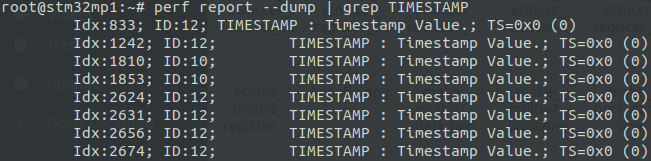
\includegraphics[width=\textwidth]{\pathPartTwo/perf_report_timestamp_0_dark}
		\caption{Extrait des trames TIMESTAMP nulles du fichier perf.data}
	    \label{fig:perf_report_timestamp_0}
	\end{center}
\end{figure}

\underline{\textbf{Note : }} On peut observer sur l'extrait ci-dessus que les
trames TIMESTAMP sont générées sur les deux processeurs, avec leur identifiant
\textbf{ID:10} et \textbf{ID:12}. \\

Cette étape n'étant qu'une étape de diagnostic du problème, une implémentation
plus élaborée et "upstreamable" doit être conçue, car tous les SoCs utilisant
ce pilote ne font pas face à ce problème. On sait que le registe
\textbf{ETMCCER} mentionné en \ref{par:timestamp} est défini lors de
l'implémentation, et possède un bit identifiant si le timestamp est supporté
par l'ETMv3. Ainsi, il faut encapsuler ce "diagnostic" dans une condition
permettant de vérifier si le timestamp est supporté. En pratique, une
structure \textbf{drvdata} est véhiculée au sein du pilote. Cette structure
contient les spécificités associées à une instance de l'ETM, telles que son
adresse d'accès ou le CPU et les horloges auxquelles il est attribué. Cette
structure spécifie également les valeurs des registres ETMCCR et ETMCCER. On
peut donc récupérer la valeur du mot \textbf{TIMSTMP} en l'isolant grâce à une
opération bit à bit. Puis, si cette valeur vaut 1, signifiant que le timestamp
est implémenté, alors on l'active dans l'ETMCR. La figure
\ref{fig:driver_etmv3_code_1} ci-dessous illustre cette implémentation.

\begin{figure}[H]
	\begin{center}
		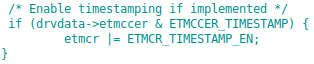
\includegraphics[scale=0.8]{\pathPartTwo/driver_etmv3_code_1}
		\caption{Extrait du code du pilote gérant l'ETMv3}
	    \label{fig:driver_etmv3_code_1}
	\end{center}
\end{figure}

Les traces Coresight présentant des paquets TIMESTAMP nuls, il faut maintenant
trouver comment avoir des valeurs incrémentées.  Après avoir consulté les
archives de mails Coresight et la documentation de l'IP, on s'aperçoit que le
registre de contrôle du compteur \textbf{TSG\_CNTCR} possède un bit EN
consacré à l'activation de l'incrémenteur du tsgen (figure
\ref{fig:tsg_cntcr_register}). Celui-ci est en en lecture/écriture et la
memory map annonce son adresse à 0x50082000.  Après vérification manuelle du
registre en utilisant \textbf{devregs} le bit EN apparaît à 0, montrant ainsi
que le compteur de l'incrémenteur est désactivé. \\

\begin{figure}[H]
	\begin{center}
		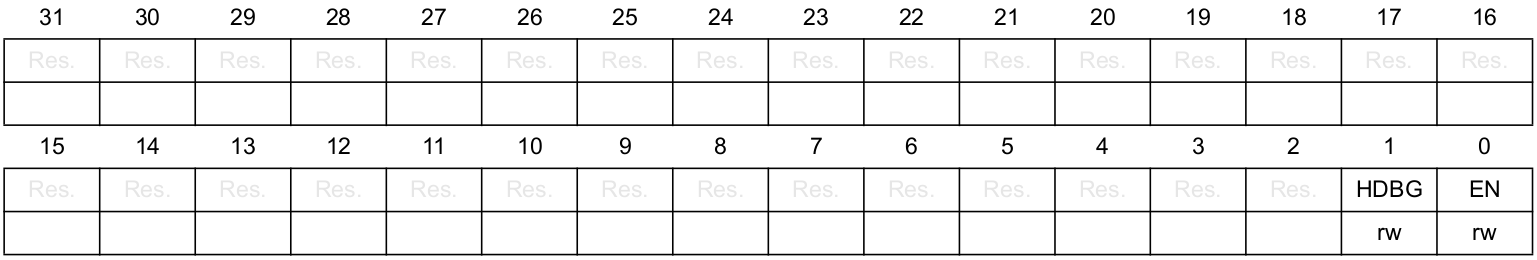
\includegraphics[width=\textwidth]{\pathPartTwo/tsg_cntcr_register_2}
		\caption{Aperçu du registre TSG\_CNTCR du Timestamp Generator}
	    \label{fig:tsg_cntcr_register}
	\end{center}
\end{figure}

Pour activer ce bit à 1, plusieurs méthodes sont possibles :

\begin{itemize}[label=\textbullet]
	\item Stopper l'exécution avant le démarrage du noyau Linux
		manuellement et passer par la console pour l'activer .
	\item Activer ce bit avec l'utilitaire devregs, toujours manuellement,
		avant l'exécution de perf record.
	\item Activer ce bit par défaut dans la configuration du système.
	\item Trouver une solution pour le faire dynamiquement.
\end{itemize}

L'idéal est d'automatiser cette activation afin que le client ait le moins
d'étapes à effectuer pour obtenir son résultat. Les deux premiers points sont
donc utilisés uniquement à des fins de validation du problème. Aussi le bit
est activé avec \textbf{devregs} avant le lancement d'une trace. Le perf.data
résultant montre que la valeur des paquets de timestamp s'incrémentent bien.
La modification du registre \textbf{TSG\_CNTCR} est donc responsable de
l'apparition de timestamps valides. \\

\begin{figure}[H]
	\begin{center}
		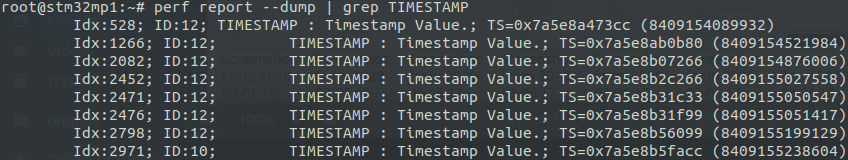
\includegraphics[width=\textwidth]{\pathPartTwo/perf_report_timestamp_dark}
		\caption{Extrait des trames TIMESTAMP du fichier perf.data}
	    \label{fig:perf_report_timestamp}
	\end{center}
\end{figure}

Ensuite, après discussion avec l'architecte du projet STM32MP15 et Mathieu
Poirier, l'activation par défaut de cette horloge n'était pas envisageable
dans un soucis de consommation superflue de la carte életronique et d'une
activation systématique malgré une utilisation ponctuelle. Il a fallu donc
trouver une solution pour activer dynamiquement cette horloge, lorsque l'IP
Coresight de l'ETMv3 est présente au sein du SoC. \\

De même, deux méthodes se présentent :

\begin{itemize}[label=\textbullet]
	\item Implémentation d'un pilote pour le tsgen.
	\item L'utilisation d'un noeud dans le device tree. \\
\end{itemize}

L'implémentation d'un pilote dédié à la gestion du générateur de timestamp est
séduisante dans la mesure où elle se base sur la détection automatique du
composant en le cherchant à travers le bus AMBA. Cela est possible puisque
tout système Coresight ne possède qu'un timestamp generator. Comme
l'activation ne concerne qu'un bit dans la configuration des registres du
tsgen, on pourrait tout aussi bien passer par un noeud arbitraire implémenté
dans le device tree. Ainsi cela permettrait aux constructeurs n'ayant pas
cette horloge par défaut de pouvoir l'activer sans crainte de gêner ceux
l'ayant par défaut. \\

\begin{figure}[H]
	\begin{center}
		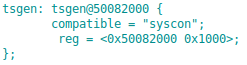
\includegraphics[scale=0.8]{\pathPartTwo/tsg_dt_property}
		\caption{Extrait du device tree, avec la propriété ajoutée}
	    \label{fig:tsg_dt_property}
	\end{center}
\end{figure}

Par mesure de simplicité, la deuxième méthode d'implémentation a été choisie.
Un noeud décrivant le timestamp generator a donc été rajouté dans le device
tree, que la figure \ref{fig:tsg_dt_property} met en valeur. En addition, une
propriété est ajoutée dans les noeuds des ETMs pour faire référence à
l'utilisation de cet IP. Cette propriété est possible grâce au pilote
MFD/syscon. C'est un framework implémenté dans le noyau dont la vocation est
d'uniformiser l'implémentation de pilotes par une API. Le pilote syscon en
particulier (SYStem CONtroller) permet ainsi un accès à divers registres de
configuration n'ayant aucun lien matériel entre eux. \\

La gestion du noeud et de la propriété dans le device tree se traite lors de
l'appel de la fonction \textbf{etm\_probe()} pendant l'initialisation du noyau
Linux. Il faut modifier cette fonction pour que la propriété soit lue, et
analyser en conséquence suivant les cas où elle ne serait pas présente dans
une autre configuration du device tree. Un booléen \textbf{tsgen\_active} est
ainsi initialisé suivant la présence ou non de cette propriété. Dans le cas où
elle est absente, aucune opération n'est réalisée. Dans le cas échéant, la
propriété pointant vers le noeud du tsgen, est alors lue et l'adresse du tsgen
est stockée dans une structure \textbf{regmap} (REGister MAP). Si la lecture
de la propriété échoue, une erreur est renvoyée comme la figure
\ref{fig:Activation_TSGEN} le met en valeur. Cette structure regmap interface
le registre \textbf{TSG\_CNTCR}, et permet au pilote de le modifier.  Ainsi
avec l'API regmap, le bit est modifié conformément à l'activation du compteur.

\begin{figure}[H]
	\begin{center}
		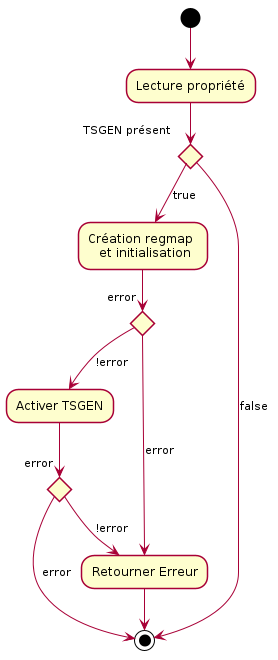
\includegraphics[scale=0.5]{\pathPartTwo/Activation_TSGEN}
		\caption{Diagramme de l'algorithme d'activation du tsgen}
	    \label{fig:Activation_TSGEN}
	\end{center}
\end{figure}

\subsection{Validation fonctionnelle et documentation}
\label{sec:validation_tests}

\subsection{Revue par les pairs}
\label{sec:peer_review}

Une fois l'implémentation effectuée, (cf figure \ref{fig:Activation_TSGEN}),
une première validation officieuse de l'implémentation par les pairs est
faite. Le code produit est soumis à Mathieu Poirier sous forme de patchs, qui
permet au développeur et mainteneurs d'échanger d'importantes quantités de
code sans les inconvénients d'envoyer tous les fichiers modifiés. \\

Après examen, Mathieu révèle qu'une solution meilleure est de créer
directement un pilote \textbf{coresight-tsg} dédié à la gestion du générateur
de timestamp. Comme c'est également le mainteneur du sous-système Coresight au
sein du noyau Linux, le code ne peut pas être upstreamé, car son aval n'est
pas approuvé compte tenu de la solution retenue.

\subsubsection{Scénarios de tests}
\label{sec:tests}

Pour valider cette fonctionnalité, des scénarios de tests sont mis en place.
Ils couvrent notamment les cas d'utilisation suivants :

\begin{itemize}[label=\textbullet]
	\item Les traces sont lancées à un espace utilisateur.
	\item Les traces sont lancées à un espace noyau.
	\item On peut enregistrer les traces sur l'ensemble des threads. 
	\item On peut enregistrer les traces sur l'ensemble des deux
		processeurs.
	\item On peut enregistrer des traces avec d'autres options de
		formatage.
	\item On peut analyser les traces brutes enregistrées.
	\item On peut analyser les traces formatées enregistrées.
\end{itemize}

Des tests nominaux sont ensuite effectués :

\begin{enumerate}
	\item perf record -e cs\_etm/@tmc\_etf0/u --per-thread ./thread
	\item perf record -e cs\_etm/@tmc\_etf0/k --all-cpus ./thread
	\item perf record -e cs\_etm/@tmc\_etf0/k --per-thread ./thread
	\item perf record -e cs\_etm/@tmc\_etf0/u --all-cpus ./thread 
\end{enumerate}

Dans les deux derniers scénarios nominaux, un affichage des données de manière
formatée ne s'effectue pas, cependant ces cas affichent bien les données
brutes. De plus, dans chaque cas les Context ID et Timestamps des traces
montrent qu'elles proviennent bien des deux processeurs. D'autres tests
couvrants plus de cas sont ensuite effectués avec différents programmes pour
s'assurer qu'ils passent bien avec divers types de programmes. Ils prennent
aussi en compte divers options de formatage en sortie et des évènements à
tracer en particulier. Un exemple de trace analysées se trouve en annexe. Les
résultats sont disponibles ci-dessous :

\begin{table}[H]
\centering
\begin{tabular}{|c|c|}
\hline
Scénario de test                                                                                             & Analyse des données \\ \hline
Scénario nominal 1                                                                                           & Brutes + formatées  \\ \hline
Scénario nominal 2                                                                                           & Brutes + formatées  \\ \hline
Scénario nominal 3                                                                                           & Brutes              \\ \hline
Scénario nominal 4                                                                                           & Brutes              \\ \hline
Traces noyau par CPU avec timestamp                                                                          & Brutes + formatées  \\ \hline
\begin{tabular}[c]{@{}c@{}}Traces noyau par CPU avec contextID\\ et formatage par instructions\end{tabular}  & Brutes + formatées  \\ \hline
\begin{tabular}[c]{@{}c@{}}Trace noyau par CPU avec timestamp \\ et formatage par branchements\end{tabular}  & Brutes + formatées  \\ \hline
\begin{tabular}[c]{@{}c@{}}Trace noyau par CPU avec timestamp \\ et avec instructions par cycle\end{tabular} & Brutes              \\ \hline
\begin{tabular}[c]{@{}c@{}}Trace utilisateur par thread \\ avec programme "uname"\end{tabular}               & Brutes + formatées  \\ \hline
\begin{tabular}[c]{@{}c@{}}Trace utilisateur par thread\\  avec programme "thread"\end{tabular}              & Brutes + formatées  \\ \hline
\end{tabular}
\end{table}

\subsubsection{Rédaction de la documentation}
\label{sec:wiki}

Enfin, une documentation doit être mise en place pour expliquer au client le
fonctionnement de Coresight, ce qu'il peut lui apporter et comment prendre en
main le framework. Un Wiki public est ainsi en cours d'élaboration au moment
où ce rapport est rédigé. Il décrit d'un côté le système d'un point de vue
matériel, le rôle des composants principaux et apporte plus de précision sur
le framework et son intégration avec perf d'un autre côté. \\

Le but de ces articles est également d'illustrer avec des examples pour que le
client puisse prendre en main le système le plus efficacement possible. Le
processus de validation de ces articles est effectué en deux temps. D'une part
des retours internes sont faits à l'aide de remarques à l'auteur de l'article
et ensuite, une fois que l'article est suffisamment élaboré pour le considérer
terminé, il est alors rendu disponible publiquement aux clients. De plus, dans
un soucis de communication universelle, les articles sont rédigés en anglais.

% perf script cs-trace-disassembly.py non existent
% https://lists.linaro.org/pipermail/coresight/2020-May/004009.html
